\section{Specifying a Graph of Lists, Maps, and Registers}\label{sec:datatypes}

We now make the OpSets approach concrete by defining example semantics for commonly-used data structures: maps (which associate values with user-specified keys) and lists (linear sequences of values).
The map datatype can also represent a set (by using keys as members of the set, and ignoring values).
The list datatype can also represent text (by mapping each character to a list element).
In both lists and maps the values may be primitives (such as numbers or strings), or references to other map or list objects.
Using these references we can construct arbitrary object graphs, including cycles of object references, like in object-oriented programming languages.
In \S~\ref{sec:tree} we will show how to restrict this object graph so that it conforms to a tree structure.

We treat each key of a map, and each element of a list, as a multi-value register.
That is, if there are several concurrent assignments to the same map key or list element, our datatype preserves all concurrently written values.
Thus, reading a map key or list element may return multiple values, which may be merged explicitly by the user.
Assigning a new value to a map key or list element overwrites all causally preceding values.
Different register behaviour, such as last-writer-wins (arbitrarily picking one of the concurrently written values as winner), can easily be defined, as we show later.

\subsection{Generating Operations}\label{sec:datatypes-gen}

An OpSet for these datatypes may contain six types of operation:
\begin{itemize}
    \item $(\mathit{id},\, \mathsf{MakeMap})$ creates a new, empty map object that is identified by $\mathit{id}$.
    \item $(\mathit{id},\, \mathsf{MakeList})$ creates a new, empty list object that is identified by $\mathit{id}$.
    \item $(\mathit{id},\, \mathsf{MakeVal}(\mathit{val}))$ associates the ID $\mathit{id}$ with the primitive value $\mathit{val}$ (e.g.\ a number, string, or boolean).
        This operation is used to ``wrap'' any primitive value, allowing $\mathsf{Assign}$ operations (see below) to always use IDs as values, regardless of whether the value is a primitive value, or a reference to a map or list object.
    \item $(\mathit{id},\, \mathsf{InsertAfter}(\mathit{ref}))$ creates a new list element with ID $\mathit{id}$, and inserts it into a list.
        If $\mathit{ref}$ is the ID of a prior $\mathsf{MakeList}$ operation, then the new element is inserted at the head of that list.
        Otherwise $\mathit{ref}$ must be the ID of an existing list element (i.e.\ a prior $\mathsf{InsertAfter}$ operation), in which case the new list element is inserted immediately after the referenced list element.
        Note that the $\mathsf{InsertAfter}$ operation does not associate a value with the new list element; that is done by a subsequent $\mathsf{Assign}$ operation.
    \item $(\mathit{id},\, \mathsf{Assign}(\mathit{obj}, \mathit{key}, \mathit{val}, \mathit{prev}))$ assigns a new value to a key within a map (if $\mathit{obj}$ is the ID of a prior $\mathsf{MakeMap}$ operation), or to a list element (if $\mathit{obj}$ is the ID of a prior $\mathsf{MakeList}$ operation).
        In the case of map assignment, $\mathit{key}$ is the user-specified key to be updated, which may be any primitive value such as a string or integer.
        In the case of a list, $\mathit{key}$ is the ID of the list element to be updated (i.e.\ the ID of a prior $\mathsf{InsertAfter}$ operation).
        $\mathit{val}$ is the ID of the value being assigned, which may identify a $\mathsf{MakeMap}$, $\mathsf{MakeList}$, or $\mathsf{MakeVal}$ operation.
        $\mathit{prev}$ is the set of IDs of prior $\mathsf{Assign}$ operations to the same key in the same object, which are overwritten by the present operation.
    \item $(\mathit{id},\, \mathsf{Remove}(\mathit{obj}, \mathit{key}, \mathit{prev}))$ removes a key-value pair from a map, or an element from a list.
        As with $\mathsf{Assign}$, $\mathit{obj}$ is the ID of the prior $\mathsf{MakeMap}$ or $\mathsf{MakeList}$ operation that created the object being updated, and $\mathit{key}$ identifies the key or list element being removed.
        $\mathit{prev}$ is the set of IDs of prior $\mathsf{Assign}$ operations to the same key in the same object, which are removed by the present operation.
\end{itemize}

\ifarxiv
  \noindent
  Pseudocode for generating these operations is given in Appendix~\ref{sect:appendix:generating-ops}.
\else
  \noindent
  Pseudocode for generating these operations is provided in an appendix of the extended version of this paper \cite{ExtendedVersion}.
\fi


\subsection{Interpreting Operations}\label{sec:datatypes-interp}

We use the sequential OpSet interpretation given in \S~\ref{sec:op-serial}.
To encode the current state of map and list data structures we use a pair of relations $(E,\, L)$:

\begin{description}
    \item[The element relation $E \subseteq (\mathrm{ID} \times \mathrm{ID} \times (\mathrm{ID} \cup \mathrm{Key}) \times \mathrm{ID})$]
        is a set of 4-tuples containing the values currently assigned to map keys and list elements.
        If $(\mathit{id}, \mathit{obj}, \mathit{key}, \mathit{val}) \in E$, then an $\mathsf{Assign}$ operation with ID $\mathit{id}$ updated the object with ID $\mathit{obj}$, assigning the value with ID $\mathit{val}$ to the map key or list element $\mathit{key}$.
        If $\mathit{obj}$ references a list object, $\mathit{key}$ is the ID of an element in the list relation $L$ (see below).
        If $\mathit{obj}$ references a map object, any primitive value such as string or integer may be used as $\mathit{key}$.
    \item[The list relation $L \subseteq (\mathrm{ID} \times (\mathrm{ID} \cup \{\bot\}))$] is a set of pairs that indicates the order of list elements.
        If $(\mathit{prev}, \mathit{next}) \in L$, that means the list element with ID $\mathit{prev}$ is immediately followed by the list element with ID $\mathit{next}$.
        We use $(\mathit{last}, \bot) \in L$ to indicate that list element $\mathit{last}$ has no successor.
        To indicate that $\mathit{head}$ is the first element in the list $\mathit{obj}$ (i.e.\ $\mathit{obj}$ is the ID of the $\mathsf{MakeList}$ operation that created the list) we have $(\mathit{obj}, \mathit{head}) \in L$.
\end{description}

\noindent
Initially, both relations are empty; that is, we have $\llbracket\emptyset\rrbracket = \mathsf{InitialState} = (\emptyset,\, \emptyset)$.
We can then define the interpretation of the six operation types as follows:
\begin{align*}
    \mathsf{interp}\big[(E,\, L),\; &(\mathit{id},\, \mathsf{Assign}(\mathit{obj}, \mathit{key}, \mathit{val}, \mathit{prev})) \big] \;=\\
    &\Big( \big\{ (\mathit{id}', \mathit{obj}', \mathit{key}', \mathit{val}') \in E \mid
    \mathit{id}' \notin \mathit{prev} \big\} \;\cup\;
    \big\{ (\mathit{id}, \mathit{obj}, \mathit{key}, \mathit{val}) \big\},\; L \Big) \\[5pt]
    %%%%%%%%%%
    \mathsf{interp}\big[(E,\, L),\; &(\mathit{id},\, \mathsf{Remove}(\mathit{obj}, \mathit{key}, \mathit{prev})) \big] \;=\\
    &\Big( \big\{ (\mathit{id}', \mathit{obj}', \mathit{key}', \mathit{val}') \in E \mid
    \mathit{id}' \notin \mathit{prev} \big\},\; L \Big) \\[5pt]
    %%%%%%%%%%
    \mathsf{interp}\big[(E,\, L),\; &(\mathit{id},\, \mathsf{InsertAfter}(\mathit{ref})) \big] \;=\\
    &\left\{
        \arraycolsep=0pt \def\arraystretch{1.2}
        \begin{array}{ll}
            (E,\, L) & \text{if } \nexists\,n.\; (\mathit{ref},\, n) \in L\\[3pt]
            \Big(E,\; \big\{ (p,n) &\;\in L \mid p \neq \mathit{ref} \big\} \;\cup\;
            \big\{ (\mathit{ref}, \mathit{id}) \big\} \;\cup\;
            \big\{ (\mathit{id}, n) \mid (\mathit{ref}, n) \in L \big\} \Big)\\
            & \text{if } \exists\,n.\; (\mathit{ref},\,n) \in L
        \end{array} \right. \\[5pt]
    %%%%%%%%%%
    \mathsf{interp}\big[(E,\, L),\; &(\mathit{id},\, \mathsf{MakeList}) \big] \hspace{21.1pt}=\;
    \Big( E,\; L \;\cup\; \big\{(\mathit{id},\, \bot)\big\}\Big) \\[1pt]
    %%%%%%%%%%
    \mathsf{interp}\big[(E,\, L),\; &(\mathit{id},\, \mathsf{MakeMap}) \big] \hspace{17.6pt}=\; (E,\; L) \\[5pt]
    \mathsf{interp}\big[(E,\, L),\; &(\mathit{id},\, \mathsf{MakeVal}(\mathit{val})) \big] \;=\; (E,\; L)
\end{align*}

The interpretation of $\mathsf{Assign}$ and $\mathsf{Remove}$ updates only $E$ and leaves $L$ unchanged; conversely, the interpretation of $\mathsf{InsertAfter}$ and $\mathsf{MakeList}$ updates only $L$.
Both the $\mathsf{Assign}$ and $\mathsf{Remove}$ interpretations remove any tuples from causally prior assignments (those whose IDs appear in $\mathit{prev}$), but leave any tuples from concurrent assignments unchanged.
This is the behaviour of a multi-value register; if a last-writer-wins register is required, the condition $\mathit{id}' \notin \mathit{prev}$ can be changed to $\mathit{obj}' \neq \mathit{obj} \;\vee\; \mathit{key}' \neq \mathit{key}$, which removes any existing tuples with the same object ID and key.

The interpretation of $\mathsf{InsertAfter}$ resembles the insertion into a linked list, as illustrated in Figure~\ref{fig:list-insert}.
For example, to interpret $(\mathit{id},\, \mathsf{InsertAfter}(\mathit{ref}))$, if we have $(\mathit{ref}, \mathit{next}) \in L$, we remove the pair $(\mathit{ref}, \mathit{next})$ from L, and add the pairs $(\mathit{ref}, \mathit{id})$ and $(\mathit{id}, \mathit{next})$ to $L$.
Thus, the new list element $\mathit{id}$ is inserted between $\mathit{ref}$ and $\mathit{next}$.

\begin{figure}
\centering
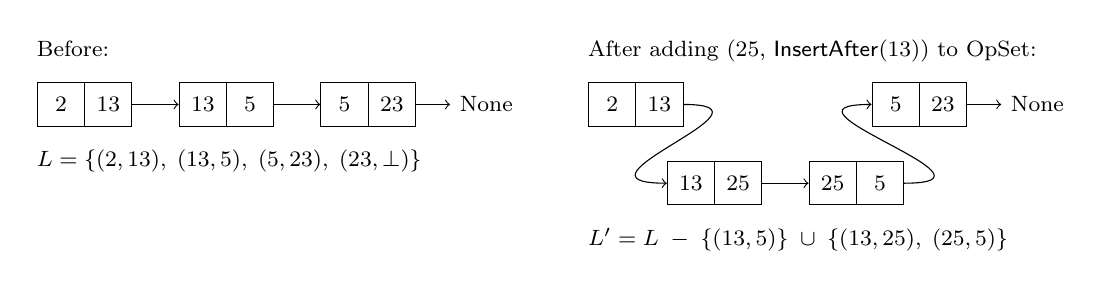
\begin{tikzpicture}
  \tikzstyle{every node}=[anchor=base,minimum width=6mm,text height=7pt,text depth=2pt,font=\footnotesize]
  \node [anchor=west] at (-7,1.7) {Before:};
  \node [anchor=west] at (-7,0.3) {$L = \{ (2, 13),\; (13, 5),\; (5, 23),\; (23, \bot) \}$};
  \node [anchor=west] at (0,1.7) {After adding $(25,\, \mathsf{InsertAfter}(13))$ to OpSet:};
  \node [anchor=west] at (0,-0.7) {$L' = L \;-\; \{(13, 5)\} \;\cup\; \{(13, 25),\; (25, 5)\}$};
    \matrix [column sep={6mm,between origins},nodes=draw,matrix anchor=west] at (-7,1) {
    \node (l1a) {2};  & \node (l1b) {13}; &&
    \node (l2a) {13}; & \node (l2b) {5};  &&
    \node (l3a) {5};  & \node (l3b) {23}; &&
    \node (l4a) [draw=none] {None}; \\
  };
  \draw [->] (l1b) -- (l2a);
  \draw [->] (l2b) -- (l3a);
  \draw [->] (l3b) -- (l4a);
  \matrix [column sep={6mm,between origins},nodes=draw,matrix anchor=west] at (1,0) {
    \node (n1) {13}; & \node (n2) {25}; &&
    \node (n3) {25}; & \node (n4) {5}; \\
  };
  \matrix [column sep={6mm,between origins},nodes=draw,matrix anchor=west] at (0,1) {
    \node (r1a) {2};  & \node (r1b) {13}; &&&&&
    \node (r3a) {5};  & \node (r3b) {23}; &&
    \node (r4a) [draw=none] {None}; \\
  };
  \draw [->] (r1b.east) .. controls (2.7,1) and (-0.3,0) .. (n1.west);
  \draw [->] (n2) -- (n3);
  \draw [->] (n4.east) .. controls (5.6,0) and (2.3,1) .. (r3a.west);
  \draw [->] (r3b) -- (r4a);
\end{tikzpicture}
\caption{Illustration of the interpretation of an $\mathsf{InsertAfter}$ operation.}\label{fig:list-insert}
\end{figure}

Note that $L$ never shrinks, it only ever grows through interpreting $\mathsf{InsertAfter}$ operations.
When a list element is removed by a $\mathsf{Remove}$ operation, the effect is that all values are removed from the list element in the element relation $E$, but the list element remains in $L$ as a \emph{tombstone}, so that any concurrent $\mathsf{InsertAfter}$ operations can still locate the referenced list position.
Thus, from a user's point of view a list element only exists if it has at least one associated value in the $E$ relation; any list elements without an associated value should be ignored.
